Dette kapitlet beskriver produktidéens gjennomførbarhet gjennom analyse av 
dens markedsverdi. Her veies produksjonskostnad opp mot salgspris og kvantitet.
Resultatene ligger til grunne for markedstilnærmelse, salg og fortjeneste. Det er 
tatt utgangspunkt i at det startes eget aksjeselskap, Autonuts AS, for salg og distribusjon av produktet 
i samarbeid med godt etablerte bedrifter.

\section{Prisestimat}
Tabell \ref{tab:price-HW} viser en oversikt over estimert kostnad for 
hardwaren som utgjør AutoNuts-systemet, og som dermed må integreres i lastebilen. Alle estimater er ekskludert tilleggskostnader som MVA og frakt.
\newline
\begin{table}[H]
\caption{Prisestimat hardwarekomponenter i Norske kroner.}
\label{tab:price-HW}
\begin{tabularx}{\textwidth}{lcc|r}
	{\bf Del} & {\bf Antall} & {\bf Pris pr. enhet} & {\bf Subtotal}\\
	\hline
	Vibrasjonssensor (piezoelektrisk accelerometer) & 6 & 14 & 84\\
	Mikrokontroller & 3 & 10 & 30\\
	Kabler & 3 & 2 & 6\\
	\hline
	\multicolumn{3}{l}{{\bf Total (NOK)}} &\multicolumn{1}{r}{120}\\
	\hline \hline
\end{tabularx} 
\end{table}

Som vist i tabellen over, estimeres det 6 vibrasjonssensorer per lastebil. Dette
tilsvarer 2 per aksling, gitt at en lastebil har 3 akslinger. Per aksling 
estimeres også én mikrokontroller, og 1 kabel. Dette gir en 
total på 120 kr. per lastebil, og en subtotal på 40 kr. per aksling. \cite{PCBmail}

Produksjonskostnaden for teamet vil, i tillegg til innkjøpsestimatet gjort 
ovenfor, være i dagsverk. Det anslås et minimum på 720 dagsverk fra 
planlegging til produksjon. Kostnadsestimatet per dagsverk er 1200 kr. Dette gir en totalkostnad for systemutviklingen på 864000 kr.

\section{Break even}
Det økonomiske målet med prosjektet er i første omgang å nå ``break even'', 
som vil si å gå i null. Figur \ref{fig:breakeven} viser forholdet mellom 
produksjons- og innstallasjonskostnad og salgsinntekter før produktet når 
vendepunktet fra underskuddsprosjekt til profitt. 
	\newline
	\begin{figure}[H]
		\centering
		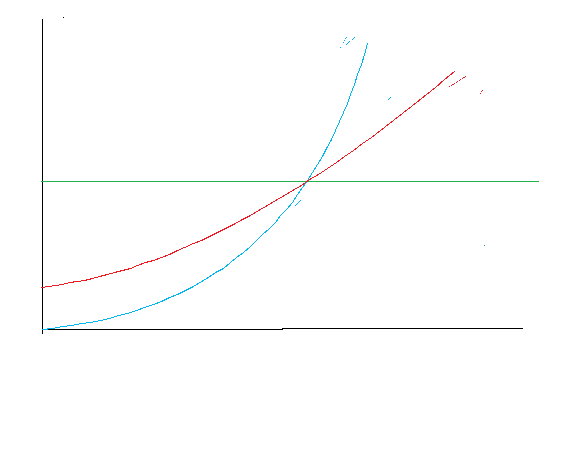
\includegraphics[width=0.80\textwidth]{images/break-even.png}
		\caption{Break even: Kostnad vs profitt.}
		\label{fig:breakeven}
	\end{figure}
X-aksen viser antall solgte ferdigmonterte enheter, mens Y-aksen viser 
Norske kroner. Rød graf er utgifter, blå graf er inntekter, mens grønn graf 
indikerer prosjektets ``break even'', altså hvor mange enheter som må selges 
før prosjektet går i overskudd.

Kongsberg Automotives representanter anbefalte en salgspris på maksimum 100 kr.
per aksling, noe som gir en total på 300 kr. per bil. Medregnet de anslåtte 
dagsverk, må det beregnes et salg på 4800 enheter før prosjektet går i overskudd. Dette 
er på mange måter et røft estimat, og vil bli påvirket av andre faktorer som leie av lokaler, 
utstyr til oppstart, drift av nettside, strøm/internett, kontorrekvisita, møblering og lønn til 
grunderne. En mer nøyaktig markedsanalyse må bli utført i samarbeid med økonom.

\section{Aksjeselskapet}
ASet vil bli opprettet av de 6 studentene bak produktet, der hver betaler inn 5000 til egenkapitalen som kreves for oppstart. 
Det kreves dog større summer for å kunne kjøpe inn utstyr og komponenter. Det vil derfor være naturlig å kontakte investorer.

\subsection{Innovasjon Norge}
Det er ikke alle som kvalifiserer seg for å få tilskudd av Innovasjon Norge, en må ha vært registrert (dvs. har organisasjonsnummer) som foretak for mindre enn tre år. Unntaksvis bedrifter som ble registrert for inntil fem år siden. 
De støtter bedrifter som trenger hjelp til forretningsmodell, nettverksbygging og forretningsutvikling. En bedrift kan derfor søke om finansiering knyttet til avklaring av forretningsideen, eller til videreutvikling inntil bedriften har oppnådd aksept i markedet. 
Tilskuddet vil normalt utgjøre 50\% av prosjektkostnadene, med en maksgrense på opptil 300 000kr per fase (Idèavklaring og markedsavklaring).18  
Innovasjon Norge gir i tillegg til tilskudd, lån og garantier til små og mellomstore bedrifter i hele landet.

\subsection{SkatteFUNN}
Bedrifter kan gjennom SkatteFUNN få skattefradrag for utgifter ved forskningsprosjekt og utviklingsprosjekt. Dette gjøres ved at inntil 20\% av kostnadene for prosjektet blir tilbakebetalt for små og mellomstore bedrifter, og inntil 18\% for store bedrifter. 
SkatteFUNN er meget fordelaktig for dette prosjektet. Det kan gjøre det mye lettere for oss ved innkjøp av komponenter og det vi trenger til produktet, da det betales skatt av dette. Siden SkatteFUNN er en statlig støtteordning på samme måte som Innovasjon Norge og det må derfor søkes om å få innvilget dette. På SkatteFUNNs egne hjemmesider kan du finne en enkel test med tre spørsmål en må besvare på for å kunne søke: 

Minitest:
 
Skal din bedrift utvikle en ny eller forbedret vare, tjeneste eller produksjonsprosess? 

Er målet med prosjektet å gi forbedret funksjonalitet og opplevelse for brukerne av en kjent løsning? 

Vet du allerede, eller tror du, at utviklingen vil kreve systematisk forskning og/eller utvikling for å få til en god løsning? 

Er svaret Ja på 1 og 3 eller 2 og 3, kan du søke SkatteFUNN.

Vårt prosjekt svarer ja på spørsmål 1 og 3, og vi vil derfor kunne søke om skattelette fra SkatteFUNN.  

\subsection{Crowdfunding}
Ved hjelp av internettsider som folk kan donere gjennom, kan folk som bryr seg om saken donere penger til bedriften. Dette er et veldig bra tilbud for små bedrifter som ikke har mye egenkapital eller jobber med en sak som involverer mange folk, og kan derfor få mange donasjoner.  
Det er snakk om relativt små donasjoner om gangen. Grunnet dette kan det ta litt vel lang tid å bygge opp kapital på denne måten, selv om det hadde vært et fint supplement for egenkapitalen. Dette vil også gi en relativt jevn inntektsstrøm gjennom oppstartsfasen, noe som vil komme godt med både til forutsette og uforutsette utgifter. 
Donasjoner gjennom Crowdfunding gir ikke noen aksjeopsjoner i bedriften, derfor vil interessen til hovedinvestorer ikke bli berørt. Det er som sagt gratis kapital, som vil nytte både selskapet og deres investorer.

\subsection{Ventureselskap}
Venturekapital er et fint tiltak for oss ettersom de ser etter selskap i etableringsfasen med stort vekstpotensial. I tillegg bidrar de ofte med kompetanse og nettverk, gjennom aktivt eierskap. Det kan være både bra og dårlig for oss ved at vi får det mye enklere i oppstartsfasen, men at de krever eierandel i selskapet. Samtidig som at de krever eierandel, har de også fem tilleggskrav for å investere penger; henholdsvis skalerbar businessmodell, voksende marked, unik idé, plan for breakeven punktet og samtidig å ha kompetanse. Det kreves da at en mer detalsjert plan for breakeven lages.

\subsection{Plan for kapital og eierandel}

Hovedinvestoren vår vil være Innovasjon Norge, vi vil søke både lån og stipend. I tillegg til Innovasjon Norge skal vi søke hos SkatteFUNN og opprette donasjonsmuligheter gjennom Crowdfunding. Gjennom disse tiltakene vil vi få nok kapital, og ved å unngå ventureselskaper kommer vi ikke til å måtte gi bort eierrettigheter, og vil da kunne bruke disse for å skaffe sammarbeidspartnere. Kapital skaffet fra investorer skal ikke benyttes som lønn. 

For å kunne overtale større bedrifter til å vurdere et samarbeid med en såpass uetablert bedrift, kan det bli nødvendig med en løsning hvor eiere i Autonuts beholder minimum 51\% av aksjene i selskapet, mens de forskjellige samarbeidspartnere vil kunne bli tildelt tilsammen opptil 49\% av selskapets aksjer.

\section{Markedsadgang}

Ettermontering av produktet vil være dyrere enn montering under produksjon av 
lastebil, man må koble fra akslingen for å montere vibrasjonssensor, samt 
trekke kabler og oppdatere software. Ettersom produktet vil bli rimeligst 
dersom det monteres under produksjon av lastebil, vil  samarbeid med en stor 
produsent, slik som feks. Volvo eller Scania være nødvendig for å entre markedet. Autonuts vil med andre ord være en egen bedrift som samarbeider med en eller flere lastebilprodusenter for å få solgt produktet. 

\section{Størrelse på marked}

Over de siste fire årene har det blitt produsert over 200 000 lasterbiler årlig 
i Europa \cite{lastebilprod-DAF}. Det vil si at markedet for produktet er 
veldig stort og Autonuts har muligheten til å komme på markedet først. I tillegg er 
det mulighet for gjøre veien tryggere, da færre hjul vil løsne på lastebiler 
som har produktet integrert.

\section{Konkurrenter}
Til nå er det ingen konkurrenter i markedet som har en digital løsning for 
automatisk deteksjon og varsling av løse hjulbolter. Det man kan finne på 
markedet i dag er manuelle løsninger, hvor man fester små indikatorer på 
boltene for å se om de har beveget seg, eller for å feste boltene bedre, som nevnt i kapittel \ref{sec:existing-solutions}.

Autonuts ønsker å inngå samarbeid med store aktører for å oppnå en nisjerolle i 
markedet. På denne måten ser vi for oss å bli den foretrukne 
underleverandøren av automatisk deteksjon og varsling av løse hjulbolter.

\section{Kundens makt}
Selv om Autonuts har fordelen med å være først ute på markedet med digital/automatisk løsning vil det være flere å konkurrere med om kundene. Dersom man er først ut i markedet vil 
man raskt kunne oppnå en god dialog med kundene. Autonuts vil etablere seg som en 
fleksibel, løsningsorientert og pålitelig leverandør. Det stilles høye krav 
til komponenter som produseres til lastebiler, siden komponentene skal være i 
drift gjennom en lang levetid. Det vil derfor være fokus på å levere produkter 
av høy kvalitet til en god pris. Med et stort fokus på 
kvalitetssikring sikrer vi at ingen produkter med feil havner hos 
sluttbruker. Autonuts ønsker fornøyde kunder og er derfor mottakelige for nye 
standarder og krav fra kundene. 

\section{Forhold til leverandører}
Det er viktig at  underleverandører som er anerkjent for å levere 
komponenter med høy kvalitet og pålitelighet velges. Samtidig må man forholde seg til 
pris på komponenter fra underleverandører, da det vil være vanskelig å få 
solgt produktet til kunder om prisen er for høy. Prøveeksemplarer fra forskjellige leverandører 
vil bli kjøpt inn og testet for å kunne sammenligne pris mot kvalitet. For å binde 
mindre kapital på lagerhold må det sikres gode og sikre avtaler med underleverandører som 
leverer komponenter på kort varsel. Det må forhandles frem langsiktige kontrakter 
for å sikre leveranse og pris, med forbehold om brudd ved mislighold av krav 
på kvalitet, pris og levering. 

\section{De fire P-ene}
\begin{description}
	\item[Produktstrategi] Etter lansering av produktet skal det jobbes med videreutvikling av produktet, så lenge det er mulig å skape verdi. Det vil da være aktuelt å se på andre problemer som kan detekteres ved bruk av 			samme sensor. Med tid vil man da kunne tilby et større produkt, og kunden vil kunne få mer 			funksjonalitet for pengene. Denne videreutviklingen vil fortsette etter de tre årene, helt til all aktuell 		funksjonalitet er implementert.
	\item[Prisstrategi] Delene som kreves for å lage produktet koster ca. 40 kr per aksling for å gjør integrering av produktet mulig. Ettersom Autonuts til en viss grad ikke har innsikt i den eventuelle samarbeidspartnerens økonomi, vil prising av produktet være opp til salgsavdelingen deres. Etter hvert som bedriften skaffer seg egenkapital vil det være naturlig å gjøre enda større avtaler med underleverandører og samarbeidspartnerer. Dette vil resultere i lavere kostnader ved innkjøp av komponenter og høyere fortjeneste ved salg.
	\item[Distribusjon og salgsstrategi] Det planlegges å selge produktet til produsenter av lastebiler, som igjen selger produktet til sine kunder som et tilleggsprodukt eller innbakt i prisen på lastebilen. 			Distribusjon vil derfor gå gjennom produsenter, og fokuset hos Autonuts vil være å inngå avtaler med 			produsenter. Salget starter først i Europa, hvor det vil være naturlig å inngå samarbeid med store europeiske produsenter slik som Volvo, Mercedez og Scania. Når salget i Europa har stabilisert seg er det ønskelig å gå videre med salg og distribusjon globalt. Et samarbeid med store produsenter, slik som Daimler \cite{daimler} er da ønskelig. Daimler er verdens største globale produsent av 				trailere over 6 tonn og produsererfor merkene Mercedez, Freightliner, Western Star, Fuso og 			BharatBenz \cite{daimler}.
	\item[Promoteringsstrategi] Autonuts planlegger å ha stand på konferanser og messer hvor hvordan vårt 	produkt kan automatisk detetektere og varsle om løse hjulbolter vil bli vist fram. Her vil det forsøkes å få kontakt med 			lastebilprodusenter og vise at Autonuts' produkt vil tjene deres produkt. Promotering av produktet vil 		inngå i kundens promotering ut til sluttbruker, da produktet vil være en del av kundens produkt. 		Både kunder og 	sluttbruker vil ha tilgang til informasjon om våre produkter gjennom vår nettside.
\end{description}
